% 
% Author: Bratin Mondal
% Roll No: 21CS10016
% Deparment of Computer Science and Engineering
% Indian Institue of Technology, Kharagpur
%

\documentclass[12pt]{article}
\usepackage{amsmath, amssymb, graphicx}
\usepackage{amsthm}  
\usepackage{float} 
\usepackage{geometry}
\usepackage{hyperref} 
\usepackage{cleveref}
\usepackage{enumitem}

\geometry{a4paper, top=0.25in, bottom=0.25in, left=0.25in, right=0.25in}  

\title{Computational Geometry (CS60064)\\ Homework Set 5}
\author{
    Bratin Mondal - 21CS10016
}
\date{}

\newtheorem{theorem}{Theorem}
\newtheorem{claim}{Claim} 

\begin{document}
\maketitle

\section*{Question 1}
\begin{enumerate}[label=(\alph*)]
    \item Give an example of 9 sites such that their Voronoi diagram has 4 vertices.
    \item Give an example of 6 sites such that the plane sweep algorithm encounters the six site events before any of the circle events. The sites should lie in general position: no three sites on a line and no four sites on a circle.
    \item Give an example where the parabola defined by some site contributes more than one arc to the beach line. Can you give an example where it contributes a linear number of arcs?
\end{enumerate}

\section*{Solution}
\paragraph{(a)}

\begin{figure}[H]
    \centering
    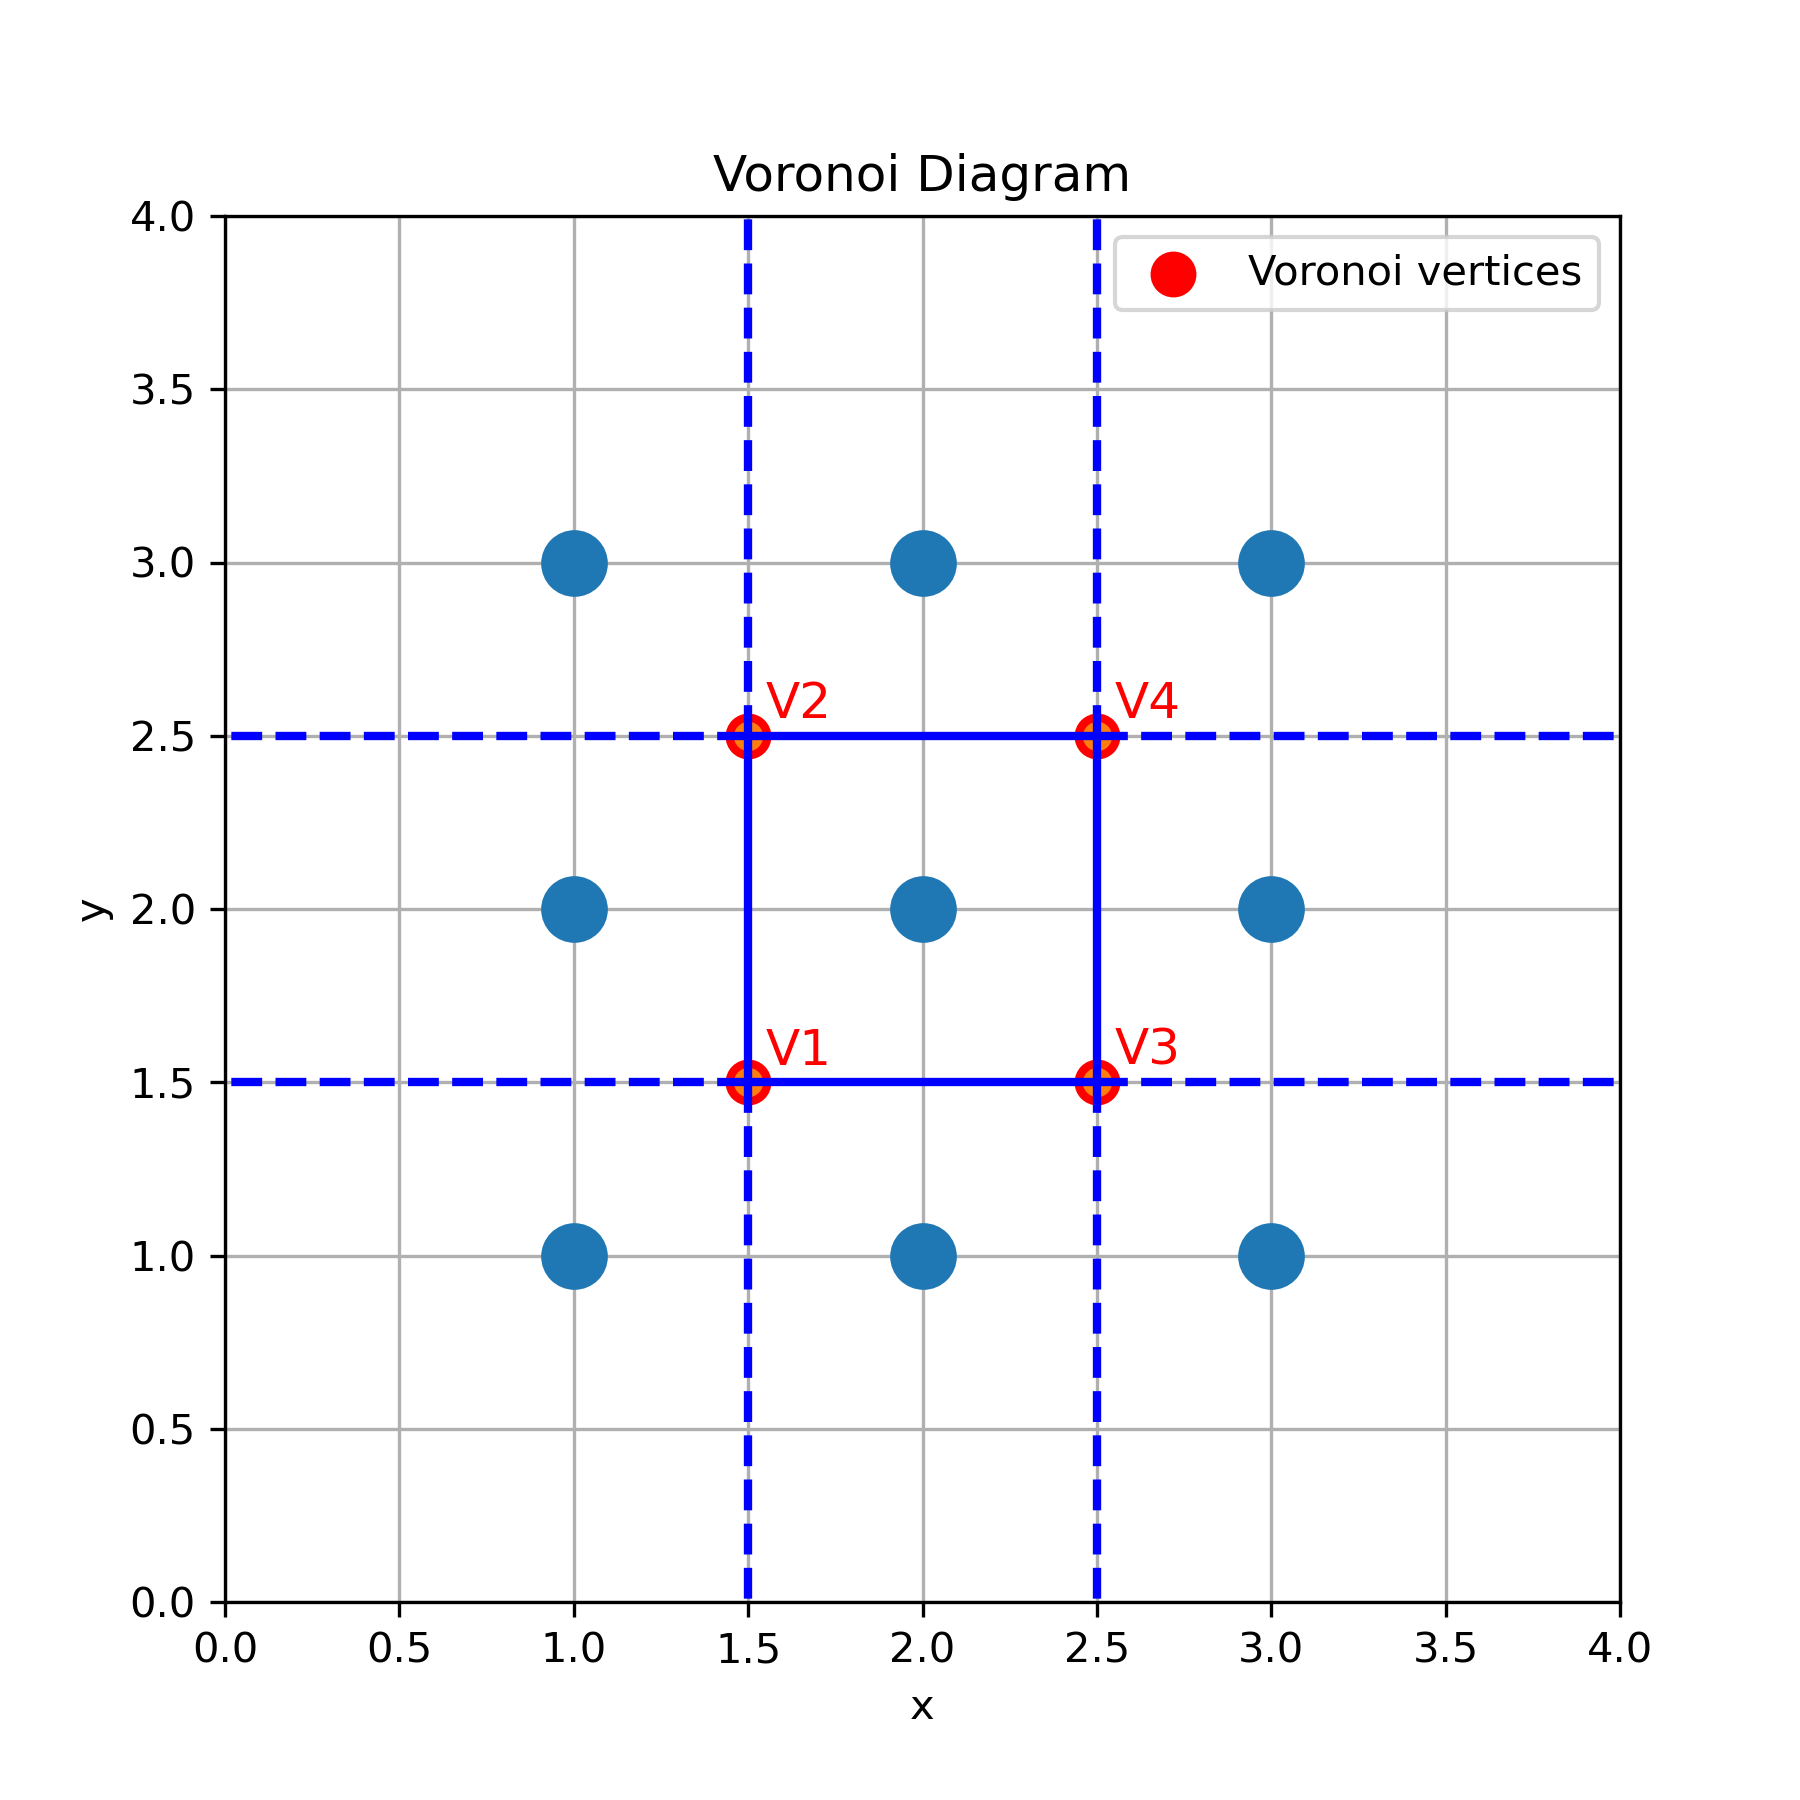
\includegraphics[width=0.5\textwidth]{img/1a.png}
    \caption{Voronoi diagram for 9 sites in a 3x3 grid.}
    \label{fig:voronoi_3x3}
\end{figure}
Consider 9 sites arranged in a 3x3 grid:
\[
(1,1),\ (1,2),\ (1,3),\ (2,1),\ (2,2),\ (2,3),\ (3,1),\ (3,2),\ (3,3).
\]
This grid produces four finite Voronoi vertices located at:
\[
(1.5, 1.5),\ (1.5, 2.5),\ (2.5, 1.5),\ (2.5, 2.5).
\]
Each of these vertices is equidistant from four neighboring sites (for example, the point \((1.5, 1.5)\) is equidistant from \((1,1)\), \((1,2)\), \((2,1)\), and \((2,2)\)). Hence, the Voronoi diagram for these 9 sites has exactly 4 vertices.

\paragraph{(b)}
We choose the six sites as follows:
\[
(2, 5),\quad (-2, 5.01),\quad (4, 4.98),\quad (-4, 4.99),\quad (6, 4.91),\quad (-6, 4.91)
\]
with the corresponding plot shown in Figure~\ref{fig:1b_sites}.

\begin{figure}[H]
    \centering
    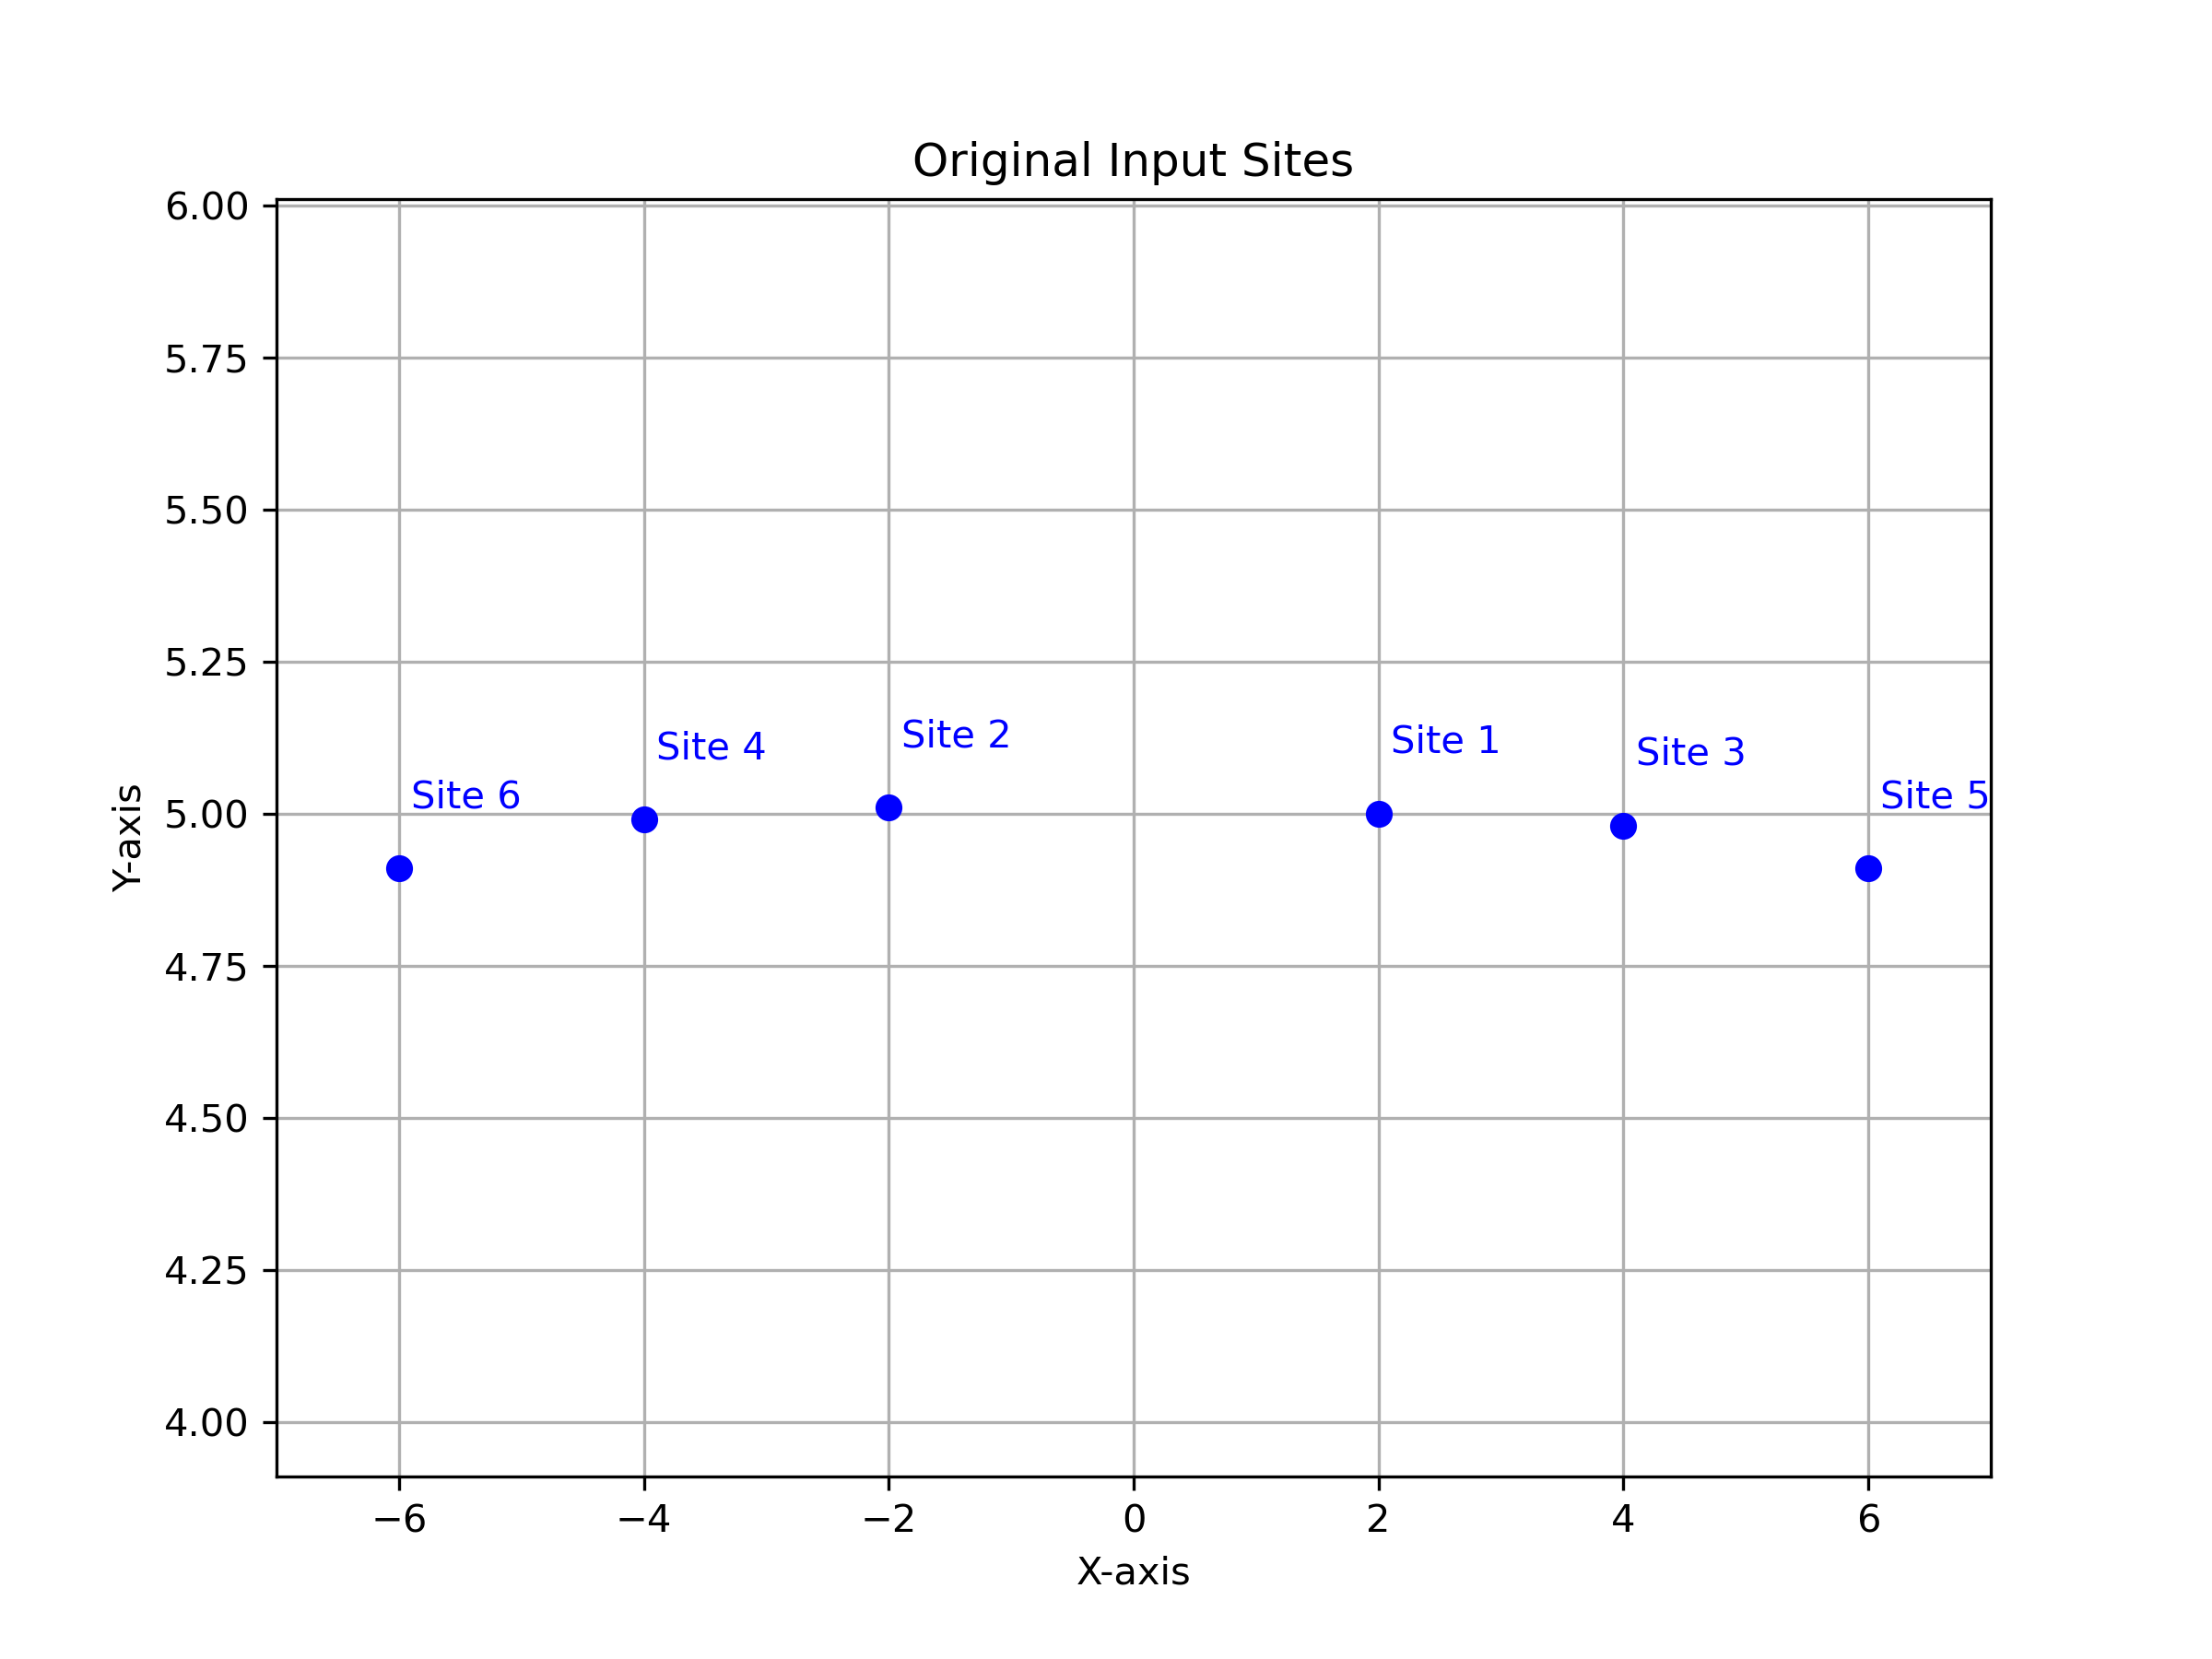
\includegraphics[width=0.5\textwidth]{img/1b.png}
    \caption{Six sites arranged for part (b).}
    \label{fig:1b_sites}
\end{figure}

The points have been chosen with the following design principles:
\begin{itemize}
    \item The differences in the $x$-coordinates are much larger compared to the differences in the $y$-coordinates. This ensures that any circle determined by three of these sites (i.e., a circle having the three sites on its boundary) will have a large radius and a center located far from the points with a large $y$-coordinate difference.
    \item The points are arranged such that for any three sites, the center of the circle defined by them is below the points. This is crucial because it guarantees that the circle events will occur only after the sweep line has encountered all the site events.
\end{itemize}

Thus, by carefully enforcing a large horizontal spread relative to the vertical spread, we guarantee that circles defined by any three sites have both a large radius and centers that are sufficiently distant (and below the points), ensuring that the circle events occur only after the sweep-line has encountered all the site events.

\paragraph{(c)}
\begin{figure}[H]
    \centering
    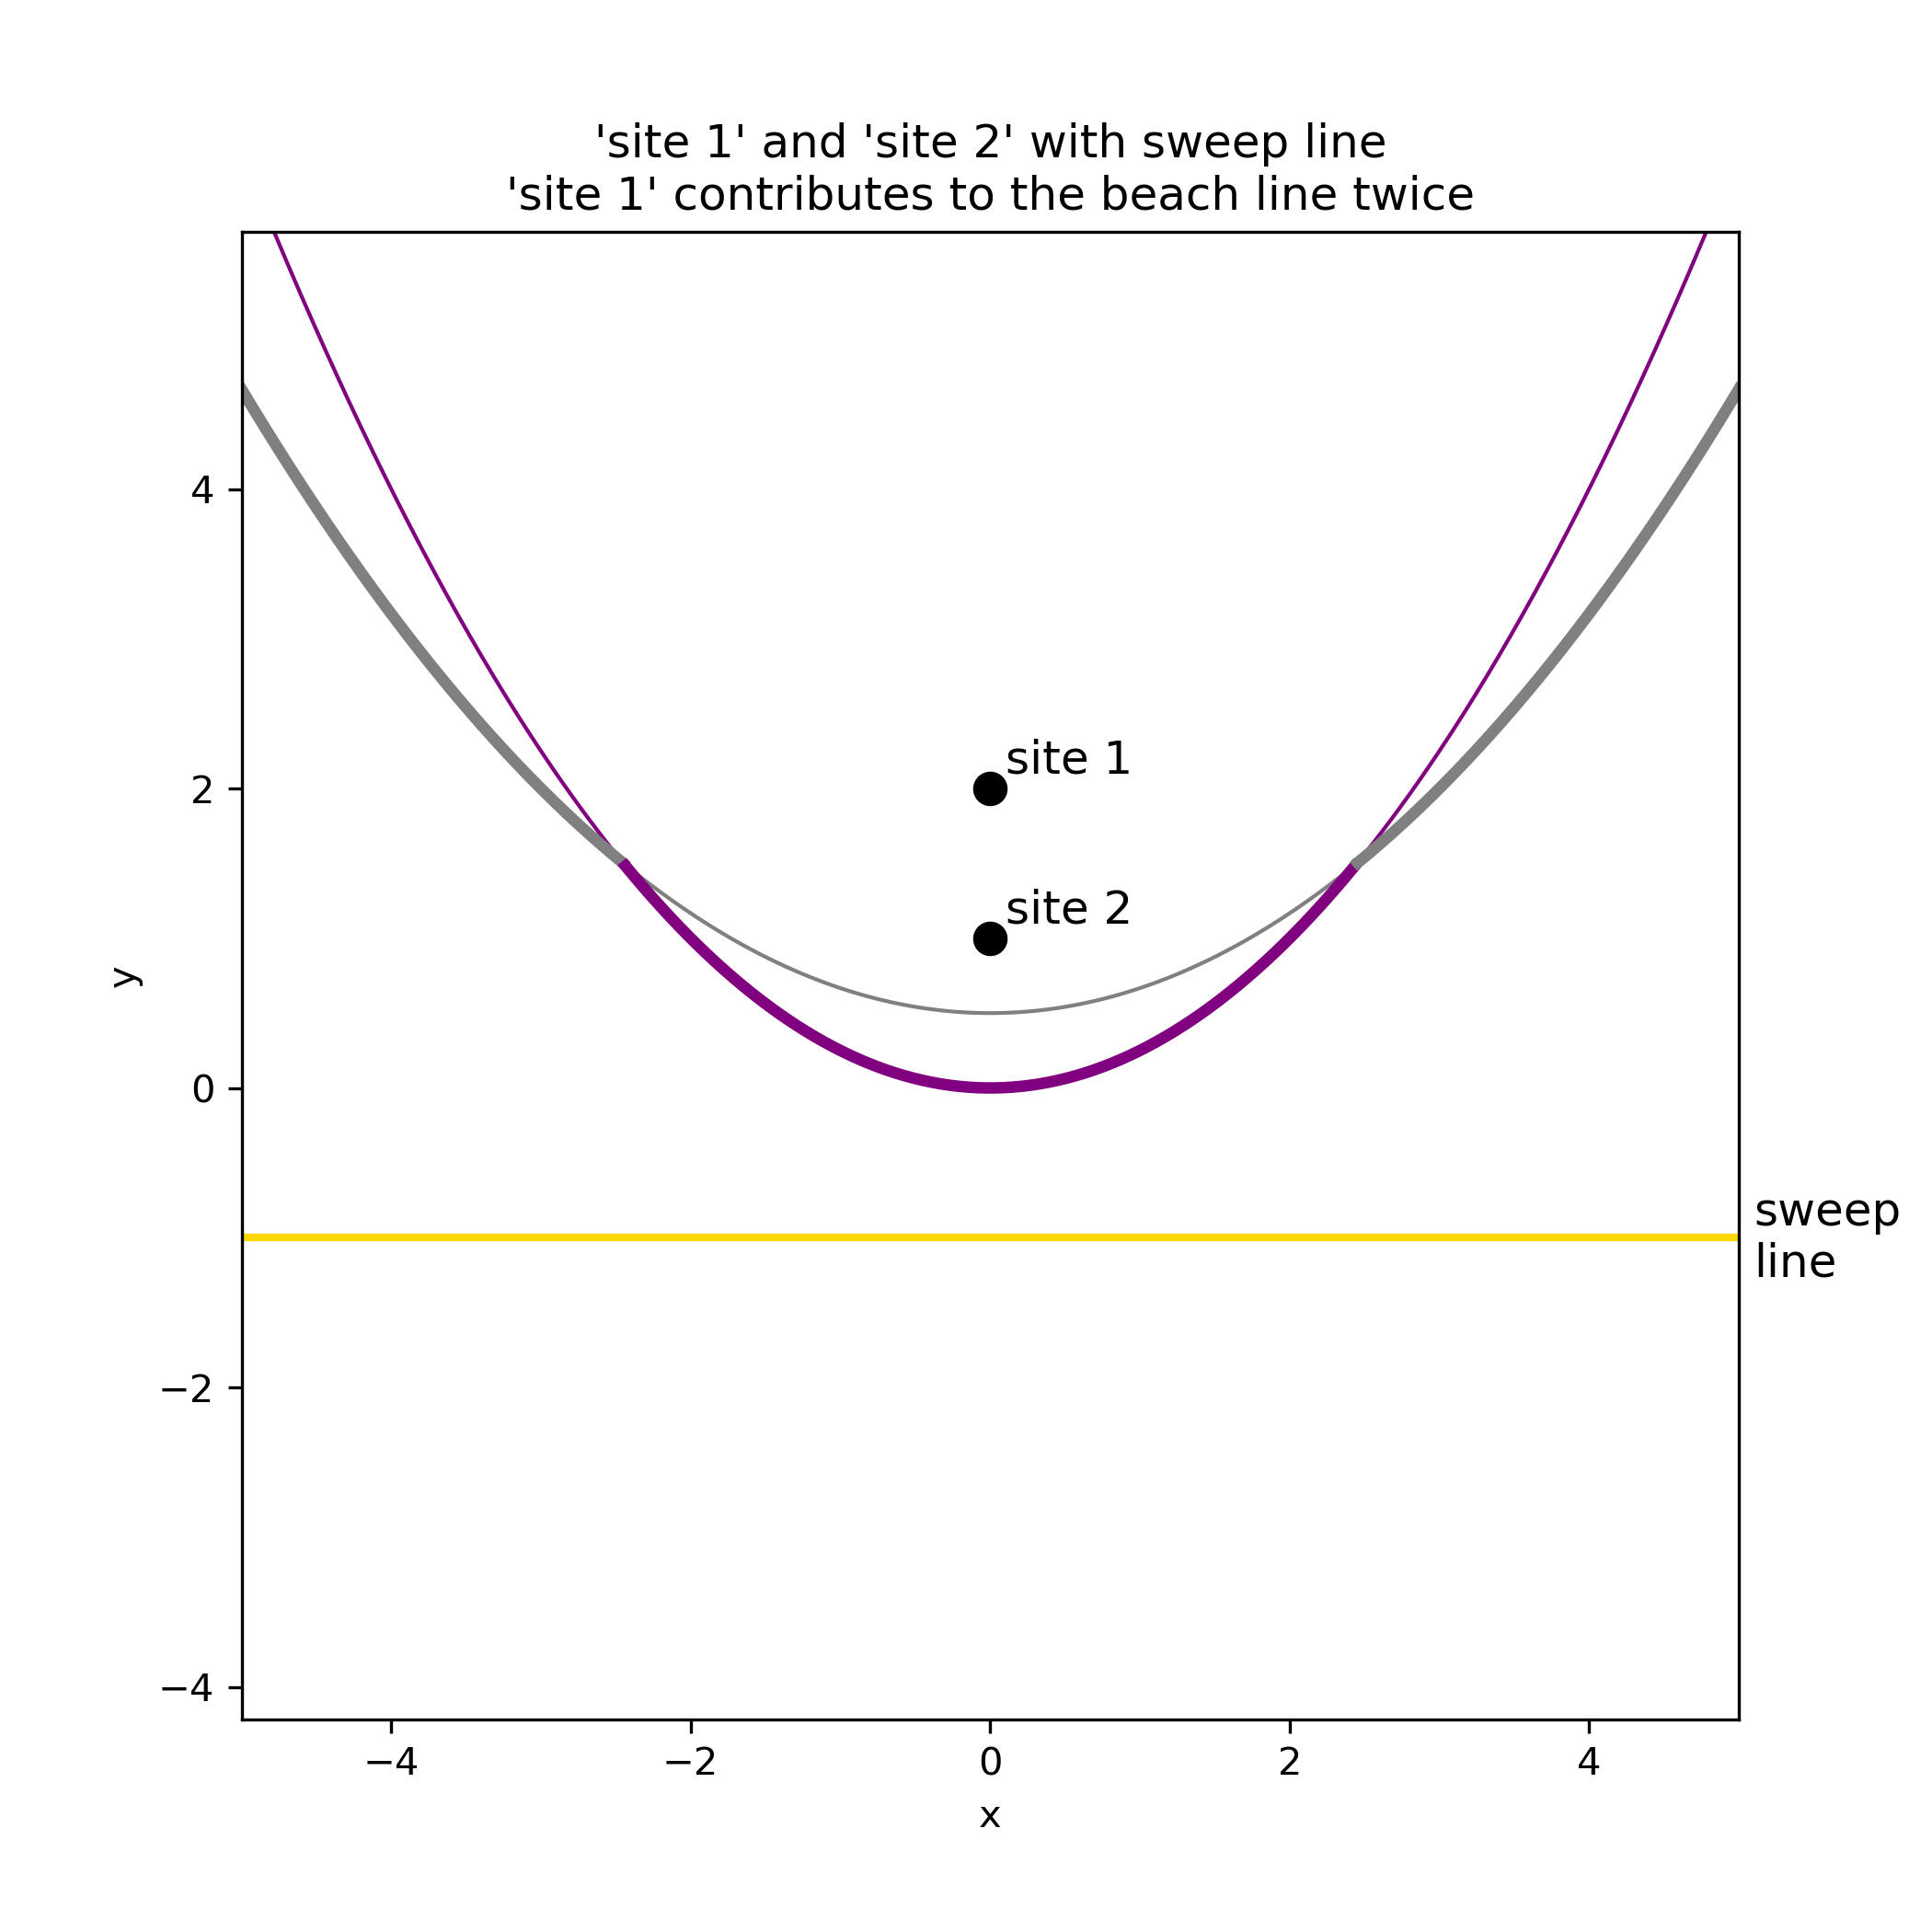
\includegraphics[width=0.5\textwidth]{img/1c_1.png}
    \caption{Parabola contributing multiple arcs.}
    \label{fig:1c_parabola}
\end{figure}
As shown in \Cref{fig:1c_parabola}, the sites are \((0,2)\) and \((0,1)\) and the sweep line is at \(y=-1\). The parabola defined by the site at \((0,2)\) contributes two arcs to the beach line.

\begin{figure}[H]
    \centering
    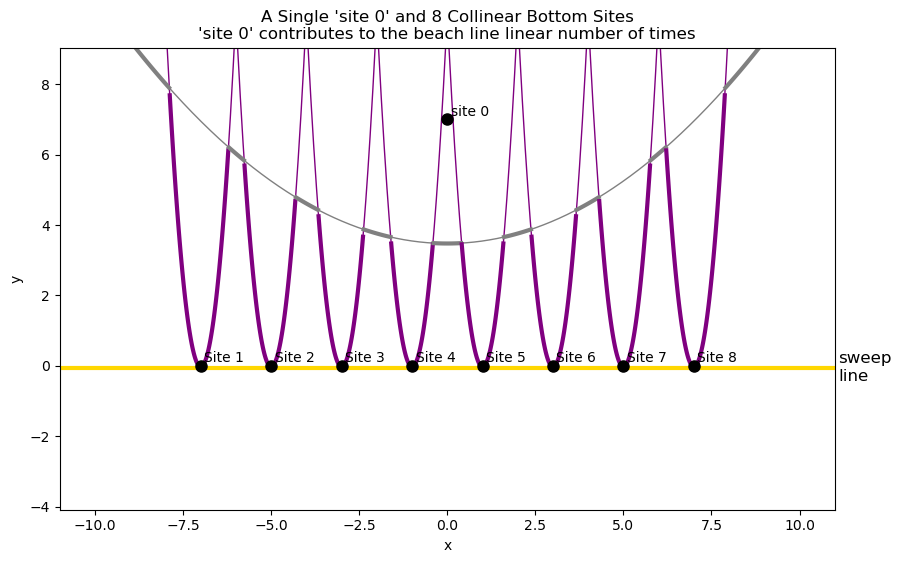
\includegraphics[width=0.5\textwidth]{img/1c_2.png}
    \caption{Parabola contributing linear number of arcs.}
    \label{fig:1c_linear_arcs}
\end{figure}
As shown in \Cref{fig:1c_linear_arcs}, the site 0 is \((0,7)\) and other sites are 
\[
(-7,0),\ (-5,0),\ (-3,0),\ (-1,0),\ (1,0),\ (3,0),\ (5,0),\ (7,0)
\]
with the sweep line at \(y=-0.05\). The parabola defined by the site at \((0,7)\) contributes \(9\) arcs to the beach line which is linear in the number of sites. We can construct a similar example for any \(n\) number of sites.
 

\section*{Question 2}
Show that $\Omega(n \log n)$ is a lower bound for computing Voronoi diagrams.

\section*{Solution}

\begin{proof}
We show that any algorithm for computing the Voronoi diagram of \(n\) sites in the plane must take \(\Omega(n \log n)\) time in the worst case by reducing the sorting problem to the computation of the Voronoi diagram.

\medskip
\noindent\textbf{Reduction from Sorting to Voronoi Diagram.}  
Suppose we are given a sequence of \(n\) real numbers 
\[
x_1, x_2, \dots, x_n.
\]
Define a mapping \(f : \mathbb{R} \to \mathbb{R}^2\) by
\[
f(x) = (x, x^2).
\]
For each \(i\), let
\[
p_i = f(x_i) = (x_i, x_i^2).
\]
The set of points 
\[
P = \{p_1, p_2, \dots, p_n\}
\]
lies on the parabola \(y = x^2\). Since the parabola is strictly convex, every point \(p_i\) lies on the boundary of the convex hull of \(P\). Moreover, when traversing the convex hull in counterclockwise order (starting from the leftmost point), the \(x\)-coordinates appear in sorted order (or in reverse order, which can be corrected). Thus, recovering the convex hull of \(P\) yields the sorted order of the original numbers.

\medskip
\noindent\textbf{Voronoi Cells and the Convex Hull.}  
We now state a classical fact.

\begin{theorem}
Let \(P\) be a set of points in the plane and let \(p \in P\). Then the Voronoi cell \(V(p)\) is unbounded if and only if \(p\) lies on the convex hull of \(P\).
\end{theorem}

\begin{proof}[Proof of Theorem]
We prove both directions:

\begin{enumerate}[label=\textbf{(\arabic*)}]
    \item \emph{If \(p\) is on the convex hull, then \(V(p)\) is unbounded.}\\[1mm]
    Since \(p\) is on the convex hull, there exists a supporting line \(L\) through \(p\) with all other points of \(P\) lying on one side of \(L\). Let \(v\) be a vector perpendicular to \(L\) that points toward the half-plane void of other points in \(P\). For any point \(q\) on the ray \(R\) emanating from \(p\) in the direction of \(v\), the distance \(d(q,p)\) is less than \(d(q,r)\) for any \(r \in P\setminus\{p\}\). Hence, \(R \subset V(p)\) and, as \(R\) is unbounded, so is \(V(p)\).
    
    \item \emph{If \(V(p)\) is unbounded, then \(p\) is on the convex hull.}\\[1mm]
    Assume for contradiction that \(p\) is not on the convex hull; that is, \(p\) lies in the interior of the convex hull of \(P\). Then for every ray \(R\) emanating from \(p\), the convexity of the hull ensures there exists some other point \(q \in P\) farther in the direction of \(R\). Consequently, for points sufficiently far along \(R\), we have \(d(q,r) < d(p,r)\), so no ray is entirely contained in \(V(p)\). This contradicts the assumption that \(V(p)\) is unbounded.
\end{enumerate}
Thus, the claim holds.
\end{proof}

\medskip
\noindent\textbf{Extracting the Sorted Order.}  
We assume that the Voronoi diagram algorithm outputs each Voronoi region as a sequence of its vertices in counterclockwise order. For the unbounded Voronoi regions, the corresponding edges will be infinite rays. We assume that the algorithm connects such edges to a vertex at infinity, which we denote as \(v_{\infty}\). 

Once the Voronoi diagram is computed, to extract the convex hull, we can follow these steps:
\begin{enumerate}[label=\arabic*.]
    \item Initialize an empty list \(H\) to store the convex hull points.
    \item Find the site \(p_{x_{\text{min}}}\) with the smallest \(x\)-coordinate. This point will be the starting point for traversing the convex hull. Set \(p_i = p_{x_{\text{min}}}\). Push \(p_i\) into \(H\).
    \item Traverse the Voronoi diagram starting from \(p_i\) and follow the edges of the Voronoi cell \(V(p_i)\) in a counterclockwise direction. During this traversal, when we encounter an edge that leads to \(v_{\infty}\), call this edge \(e_{\text{in}}\). The next edge we encounter will be \(e_{\text{out}}\). We set \(p_i\) to the site corresponding to the other face of the Voronoi diagram that is adjacent to \(e_{\text{out}}\).
    \item Continue this process until we reach the point with highest \(x\)-coordinate, which we denote as \(p_{x_{\text{max}}}\). This point will be the last point in the convex hull. Push \(p_{x_{\text{max}}}\) into \(H\).
    \item Once the points have been added, we can now traverse \(H\) to confirm the order and extract the final convex hull points.
\end{enumerate}

As we already noted that \(H\) contains the points in counterclockwise order, we can simply output the points in \(H\) to get the sorted order of the original numbers \(x_i\).


\medskip
\noindent\textbf{Complexity Argument.}  
Suppose there exists an algorithm that computes the Voronoi diagram in time
\[
T(n) = o(n \log n).
\]
Since both the mapping \(f\) takes \(O(n)\) time and the extraction of the convex hull needs us to traverse faces corresponding to every site once only and every edge is traversed at most twice, the total time for this step is also \(O(n)\) since the number of edges is at most \(O(n)\). Thus, the total time for the Voronoi diagram algorithm is:
\[
T(n) + O(n) = o(n \log n)
\]
time. This contradicts the \(\Omega(n \log n)\) lower bound for comparison-based sorting.

\medskip
\noindent\textbf{Conclusion.}  
Thus, any algorithm that computes the Voronoi diagram in the Euclidean plane must have a worst-case time complexity of \(\Omega(n \log n)\).
\end{proof}

\end{document}